\documentclass[10pt,a4paper]{article}
\usepackage[margin=2cm]{geometry}
\usepackage[T1]{fontenc}
\usepackage{lmodern}
\usepackage{amsmath,amssymb}
\usepackage{booktabs,array,tabularx}
\usepackage{enumitem}
\usepackage[dvipsnames]{xcolor}
\usepackage{tikz}
\usetikzlibrary{arrows.meta,positioning,calc,fit,backgrounds}
\usepackage[most]{tcolorbox}
\usepackage[hidelinks]{hyperref}

\setlist{nosep,leftmargin=1.2em}
\setlength{\parindent}{0pt}
\setlength{\parskip}{4pt}

\newcommand{\code}[1]{\texttt{\detokenize{#1}}}
\newtcolorbox{keybox}[1]{colback=white,colframe=black!60,coltitle=black,colbacktitle=black!8,fonttitle=\bfseries,title=#1,boxrule=0.6pt,arc=1mm,left=4pt,right=4pt,top=2pt,bottom=2pt}
\newtcolorbox{notebox}{colback=white,colframe=black!60,boxrule=0.6pt,arc=1mm,left=4pt,right=4pt,top=2pt,bottom=2pt}

\tikzset{
  blk/.style={draw,thick,minimum height=8mm,minimum width=12mm,align=center,fill=white,font=\small},
  sum/.style={draw,thick,circle,minimum size=5mm,inner sep=0pt,fill=white},
  sig/.style={-{Latex[length=2mm]},thick},
  lbl/.style={font=\scriptsize},
  plant/.style={blk,fill=green!6},
  ctrl/.style={blk,fill=blue!5},
  ffb/.style={blk,fill=orange!10},
}

\title{\textbf{Pole placement for the CNC plotter}\\[2pt]
\large design guide: workflow, design A and its parameters}
\author{scripts: \code{scripts/control/pp_design}}
\date{}

\begin{document}
\maketitle
\vspace{-6mm}

\begin{keybox}{What this document covers}
\begin{enumerate}
  \item \textbf{The workflow in short} (Sec.~\ref{sec:workflow}): which script does what, including the tools for
        tuning by hand (\code{design_B}, \code{check_design}, \code{tune_poles}, \code{explore_poles}).
  \item \textbf{Plant and controller} (Sec.~\ref{sec:plant}--\ref{sec:ctrl}): the simulated motor with friction and
        delay, the control law and its block diagram.
  \item \textbf{Design A} (Sec.~\ref{sec:designA}--\ref{sec:result}), the core of the method: pole pattern, gains,
        every parameter and requirement with its justification, the search and the final numbers.
\end{enumerate}
\end{keybox}

%==========================================================================================
\section{The workflow at a glance}\label{sec:workflow}

\begin{center}
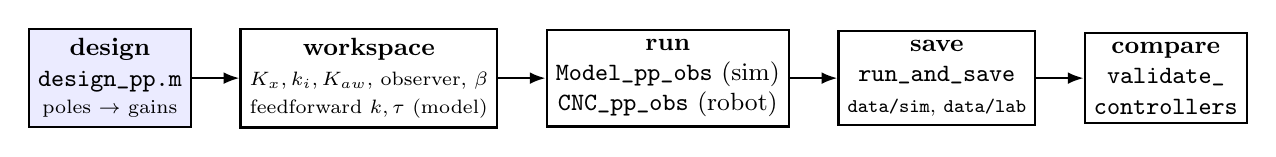
\begin{tikzpicture}[node distance=7mm and 6mm]
  \node[blk,fill=blue!8] (des) {\textbf{design}\\ \code{design_pp.m}\\[-1pt]\scriptsize poles $\to$ gains};
  \node[blk,right=of des] (ws) {\textbf{workspace}\\ \scriptsize $K_x,k_i,K_{aw}$, observer, $\beta$\\[-1pt]\scriptsize feedforward $k,\tau$ (model)};
  \node[blk,right=of ws] (sim) {\textbf{run}\\ \code{Model_pp_obs} (sim)\\ \code{CNC_pp_obs} (robot)};
  \node[blk,right=of sim] (save) {\textbf{save}\\ \code{run_and_save}\\ \scriptsize\code{data/sim}, \code{data/lab}};
  \node[blk,right=of save] (cmp) {\textbf{compare}\\ \code{validate_}\\ \code{controllers}};
  \draw[sig] (des) -- (ws); \draw[sig] (ws) -- (sim); \draw[sig] (sim) -- (save); \draw[sig] (save) -- (cmp);
\end{tikzpicture}
\end{center}

\textbf{Steps.}
\begin{enumerate}
  \item \code{tools/observer_study.m}: list the candidate designs, check them and simulate each one
        (report in \code{data/sim}).
  \item \code{tools/analyze_study.m}: accept the designs within the tolerances and rank them by error.
        For the plots and the comparison with the PID use \code{validate_controllers.m}.
  \item \code{design_pp.m}: copy the chosen design into section 1 (poles, observer, requirements) and run it
        with the search off (Sec.~\ref{sec:choose}): requirement table and Simulink variables.
  \item Run \code{CNC_pp_obs} on the robot (or \code{Model_pp_obs} to re-check) and save the run with
        \code{run_and_save}.
\end{enumerate}

\textbf{The other scripts} (folder \code{tools/}: exploration and tuning by hand; same gains, observer and requirements):

\begin{tabularx}{\linewidth}{@{}l X@{}}
\toprule
script & use \\
\midrule
\code{design_pp.m} & \textbf{main script}: the chosen design, requirement table, Simulink variables (search optional) \\
\code{observer_study.m} & comparison of many designs: requirements and one simulation each, report \\
\code{analyze_study.m} & reads the report, applies the tolerances, ranks the designs by error \\
\code{design_B.m} & three real poles $-\lambda_1,-\lambda_2,-\lambda_3$, each moved on its own by the search. No
  oscillating mode but a slower rise; it served as a step towards design A and is kept for comparison \\
\code{check_design.m} & poles given by hand (pattern A or the three poles per motor), no search: only checks and
  writes them \\
\code{tune_poles.m} & sliders for $\omega_n,\zeta,\alpha$ on both motors; \emph{lock alpha} keeps the integral pole fixed \\
\code{explore_poles.m} & drag the three poles of one motor and watch step, voltage and Bode live \\
\code{utils/} & \code{pp_setup} (models, requirements), \code{pp_gains} (poles $\to$ gains, observer),
  \code{closed_loop} (simulation with delay), \code{pp_check}, \code{pp_search}, \code{pp_report},
  \code{pp_simulink} (workspace variables) \\
\bottomrule
\end{tabularx}

%==========================================================================================
\section{Plant model and simulated plant}\label{sec:plant}

\textbf{Model used by the controller} (one per joint, identified with the linkage attached, angle in encoder degrees):
\begin{equation}
  \tau\ddot\theta + \dot\theta = b\,u,\qquad G(s)=\frac{b}{s(\tau s+1)},\qquad b=-\frac{180}{\pi}k,
\end{equation}
\begin{equation}
  x=\begin{bmatrix}\theta\\ \omega\end{bmatrix},\quad
  A=\begin{bmatrix}0&1\\0&-1/\tau\end{bmatrix},\quad
  B=\begin{bmatrix}0\\ b/\tau\end{bmatrix},\quad
  C=\begin{bmatrix}1&0\end{bmatrix}.
\end{equation}
$k,\tau$ = \code{k_xxxx_load}, \code{tau_xxxx_load} ($k\approx1.44/1.38$~rad/(V\,s), $\tau\approx0.037$~s, so the mechanical
pole is $1/\tau\approx27$~rad/s). The minus sign in $b$ is the encoder convention (a positive voltage gives a negative angle).

\textbf{Simulated plant} (\code{motor model xxxx} in the \code{Model_*} files). To test the controller against a plant
that is \emph{not} its model, \code{parameters.m} (section 5) provides a ``realistic'' plant from the multisine fit with
delay and Coulomb friction:
\begin{equation}
  u_m(t) = u_{sat}(t-T_d) - V_c\tanh\!\left(\frac{\omega_m}{w_\varepsilon}\right),\qquad
  \omega_m = \frac{k_p}{\tau_p s+1}\,u_m,\qquad \theta = -\frac{180}{\pi}\int\omega_m\,dt .
\end{equation}

\begin{center}
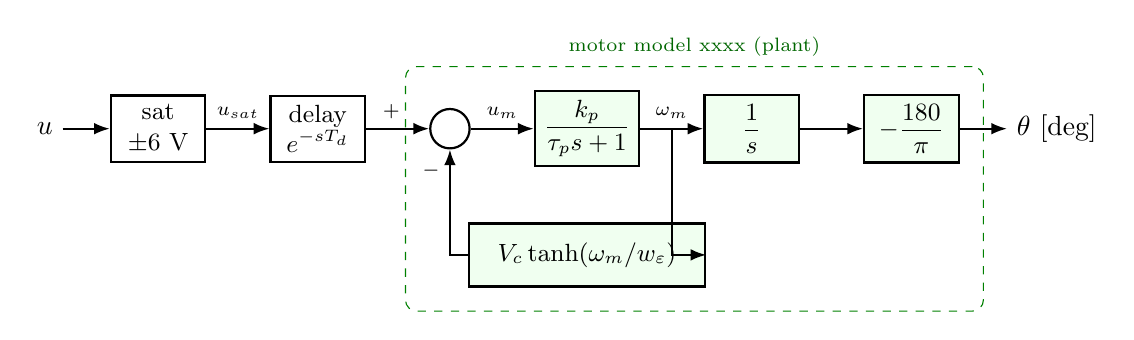
\begin{tikzpicture}[node distance=6mm and 8mm]
  \node (in) {$u$};
  \node[blk,right=6mm of in] (sat) {sat\\ $\pm6$ V};
  \node[blk,right=of sat] (del) {delay\\ $e^{-sT_d}$};
  \node[sum,right=of del] (s1) {};
  \node[plant,right=of s1] (tf) {$\dfrac{k_p}{\tau_p s+1}$};
  \node[plant,right=of tf] (int) {$\dfrac1s$};
  \node[plant,right=of int] (g) {$-\dfrac{180}{\pi}$};
  \node[right=6mm of g] (out) {$\theta$ [deg]};
  \node[plant,below=7mm of tf,minimum width=30mm] (fr) {$V_c\tanh(\omega_m/w_\varepsilon)$};
  \draw[sig] (in) -- (sat); \draw[sig] (sat) -- node[lbl,above]{$u_{sat}$} (del);
  \draw[sig] (del) -- node[lbl,above,pos=0.4]{$+$} (s1);
  \draw[sig] (s1) -- node[lbl,above]{$u_m$} (tf);
  \draw[sig] (tf) -- node[lbl,above]{$\omega_m$} coordinate[midway](om) (int);
  \draw[sig] (int) -- (g); \draw[sig] (g) -- (out);
  \draw[sig] (om) |- (fr.east);
  \draw[sig] (fr.west) -| node[lbl,left,pos=0.9]{$-$} (s1.south);
  \begin{scope}[on background layer]
    \node[draw,dashed,green!50!black,rounded corners,fit=(s1)(tf)(int)(g)(fr),inner sep=3mm,
          label={[lbl,green!40!black]above:motor model xxxx (plant)}] {};
  \end{scope}
\end{tikzpicture}
\end{center}

\begin{tabularx}{\linewidth}{@{}l c c X@{}}
\toprule
\code{use_real_plant} & $k_p,\ \tau_p$ & $T_d,\ V_c$ & meaning \\
\midrule
\code{false} & $k,\ \tau$ (= model) & 0, 0 & plant = model: checks the design itself \\
\code{true}  & 1.77/1.74,\ 0.043/0.044 s & 3.5 ms,\ 0.12/0.14 V & plant $\neq$ model, as on the bench \\
\bottomrule
\end{tabularx}

\begin{notebox}
\textbf{Where friction and delay live.} Friction and $k_p,\tau_p$ belong to the \emph{plant} (motor model subsystem):
the friction depends on the real speed $\omega_m$ and opposes it. The block computing $V_c\tanh(\cdot)$ uses the output of the
strictly proper block $k_p/(\tau_p s+1)$, so there is no algebraic loop. \code{scripts/update_models.m} adds them to
\code{Model_pp_obs} and \code{Model_pid_ff}. The delay $T_d$ belongs to the plant too and must not be copied into the
\code{CNC_*} models, where the real motor provides it.
\end{notebox}

%==========================================================================================
\section{Control law and controller block}\label{sec:ctrl}

Only $\theta$ is measured: a Luenberger observer gives $\hat x=[\hat\theta,\hat\omega]^T$. With the reference
$\phi$ (degrees) and its derivatives $\dot\phi,\ddot\phi$ (rad/s, rad/s$^2$) from the inverse kinematics:
\begin{equation}\label{eq:law}
  u = \underbrace{-K_x\left(\hat x - x_{ref}\right)}_{\text{state feedback}}
      \;\underbrace{-\,k_i e_I}_{\text{integral}}
      \;\underbrace{-\frac{1}{k}\dot\phi - \frac{\tau}{k}\ddot\phi}_{\text{feedforward}}
      \;\underbrace{-\,V_{c}\tanh\!\left(\frac{\dot\phi}{w_\varepsilon}\right)}_{\text{friction compensation}},
  \qquad x_{ref}=\begin{bmatrix}\beta\phi\\ \tfrac{180}{\pi}\dot\phi\end{bmatrix},
\end{equation}
\begin{equation}
  \dot e_I = \phi - y + K_{aw}(u_{sat}-u),\qquad
  \dot{\hat x} = A_{obs}\hat x + B_{obs}\begin{bmatrix}u_{sat}\\ y\end{bmatrix},\quad A_{obs}=A-LC,\ B_{obs}=[B\ \ L].
\end{equation}

\begin{center}
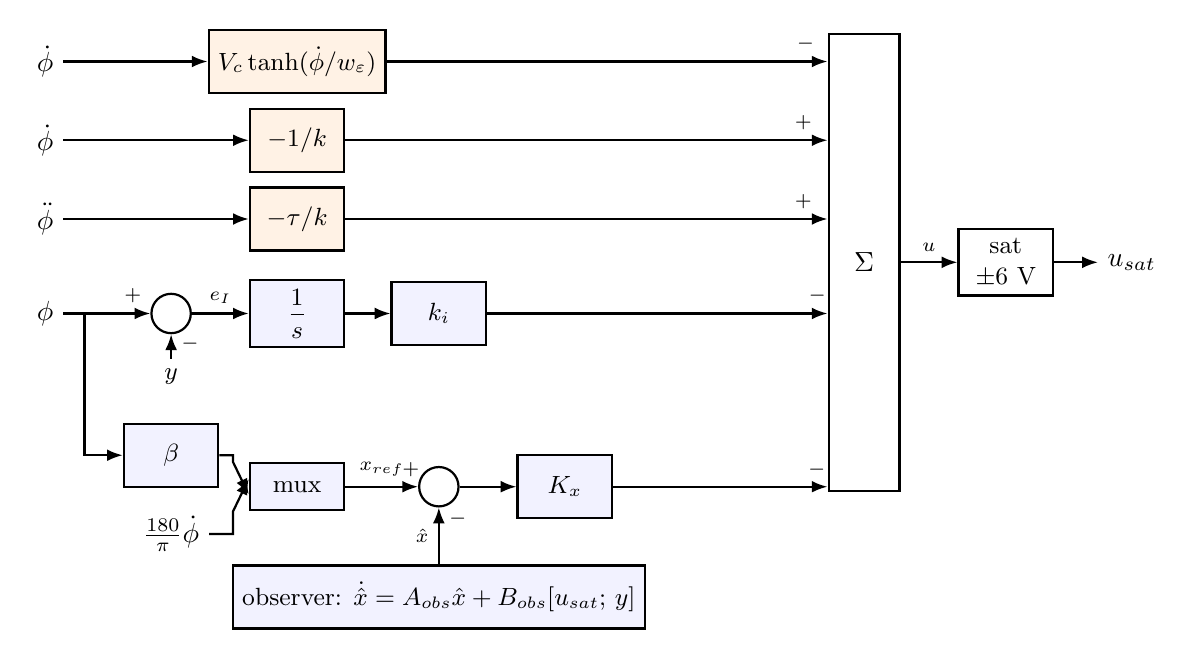
\begin{tikzpicture}
  % big summing block: every branch enters from the left with its sign
  \node[draw,thick,minimum width=9mm,minimum height=58mm,fill=white] (su) at (10.4,-0.35) {$\Sigma$};
  % feedforward rows (orange, outside the loop)
  \node (dphi0) at (0,2.2) {$\dot\phi$};
  \node[ffb] (fc) at (3.2,2.2) {$V_{c}\tanh(\dot\phi/w_\varepsilon)$};
  \node (dphi1) at (0,1.2) {$\dot\phi$};
  \node[ffb] (kv) at (3.2,1.2) {$-1/k$};
  \node (ddphi) at (0,0.2) {$\ddot\phi$};
  \node[ffb] (ka) at (3.2,0.2) {$-\tau/k$};
  % integral row
  \node (phi) at (0,-1.0) {$\phi$};
  \node[sum] (se) at (1.6,-1.0) {};
  \node[ctrl] (int) at (3.2,-1.0) {$\dfrac1s$};
  \node[ctrl] (ki) at (5.0,-1.0) {$k_i$};
  \node (yin) at (1.6,-1.8) {\small $y$};
  % state feedback row
  \node[ctrl] (beta) at (1.6,-2.8) {$\beta$};
  \node (dref) at (1.6,-3.8) {$\tfrac{180}{\pi}\dot\phi$};
  \node[ctrl,minimum height=6mm] (mux) at (3.2,-3.2) {mux};
  \node[sum] (sx) at (5.0,-3.2) {};
  \node[ctrl] (kx) at (6.6,-3.2) {$K_x$};
  \node[ctrl] (obs) at (5.0,-4.6) {observer: $\dot{\hat x}=A_{obs}\hat x+B_{obs}[u_{sat};\,y]$};
  % output
  \node[blk] (sat) at (12.2,-0.35) {sat\\ $\pm6$ V};
  \node (u) at (13.8,-0.35) {$u_{sat}$};
  % wires
  \draw[sig] (dphi0) -- (fc);  \draw[sig] (fc.east)  -- node[lbl,above,pos=0.95]{$-$} (fc.east -| su.west);
  \draw[sig] (dphi1) -- (kv);  \draw[sig] (kv.east)  -- node[lbl,above,pos=0.95]{$+$} (kv.east -| su.west);
  \draw[sig] (ddphi) -- (ka);  \draw[sig] (ka.east)  -- node[lbl,above,pos=0.95]{$+$} (ka.east -| su.west);
  \draw[sig] (phi) -- node[lbl,above,pos=0.8]{$+$} (se);
  \draw[sig] (yin) -- node[lbl,right,pos=0.6]{$-$} (se);
  \draw[sig] (se) -- node[lbl,above]{$e_I$} (int);
  \draw[sig] (int) -- (ki);
  \draw[sig] (ki.east) -- node[lbl,above,pos=0.97]{$-$} (ki.east -| su.west);
  \draw[sig] (0.5,-1.0) |- (beta.west);
  \draw[sig] (beta.east) -| ([xshift=-2mm]mux.north west) -- ([yshift=-1mm]mux.north west |- mux.west);
  \draw[sig] (dref.east) -| ([xshift=-2mm]mux.south west) -- ([yshift=1mm]mux.south west |- mux.west);
  \draw[sig] (mux) -- node[lbl,above]{$x_{ref}$} node[lbl,above,pos=0.9]{$+$} (sx);
  \draw[sig] (obs.north) -- node[lbl,left,pos=0.5]{$\hat x$} node[lbl,right,pos=0.8]{$-$} (sx);
  \draw[sig] (sx) -- (kx);
  \draw[sig] (kx.east) -- node[lbl,above,pos=0.95]{$-$} (kx.east -| su.west);
  \draw[sig] (su) -- node[lbl,above]{$u$} (sat);
  \draw[sig] (sat) -- (u);
\end{tikzpicture}
\end{center}
Blocks in orange: the feedforward, outside the loop; blue: the loop designed by pole placement. Not drawn: the
anti-windup term $K_{aw}(u_{sat}-u)$, added to the input of the integrator. The same structure is in
\code{pp + luenberg xxxx} of \code{Model_pp_obs} and \code{CNC_pp_obs}; the PID models have the same orange branch.

\begin{tabularx}{\linewidth}{@{}l X@{}}
\toprule
block & role \\
\midrule
feedforward & the voltage the nominal motor needs to follow $\dot\phi,\ddot\phi$, with the same $k,\tau$ as the controller (\code{pp_simulink} writes them into \code{k_xxxx_load}, \code{tau_xxxx_load}, read by the Gain blocks): the feedback only corrects errors \\
friction comp. & $V_{c}\tanh(\dot\phi/w_\varepsilon)$ from the \emph{reference} speed; $\tanh$ instead of $\mathrm{sign}$ avoids a voltage jump at zero speed \\
integral $k_i$ & removes constant errors (friction, load, errors in $k$); $K_{aw}=-\overline{|p|}/k_i$ unloads it when the amplifier saturates \\
$K_x$, $\beta$ & state feedback on $\hat x-x_{ref}$; $\beta$ weights the position reference (Sec.~\ref{sec:beta}) \\
observer & estimates $\omega$ from $\theta$ and the voltage really applied ($u_{sat}$) \\
\bottomrule
\end{tabularx}

%==========================================================================================
\section{Design A: pole pattern and gains}\label{sec:designA}

With $\hat x=x$ and states $z=[\theta,\omega,e_I]^T$, the loop is $\dot z=(A_i-B_iK)z$ with
$A_i=\begin{bmatrix}A&0\\-C&0\end{bmatrix}$, $B_i=\begin{bmatrix}B\\0\end{bmatrix}$, $K=[k_1\ k_2\ k_i]$.
Its characteristic polynomial and the gains that place the poles (polynomial matching; \code{acker}, Ackermann's
formula \cite{Ackermann1972}, gives the same \cite{AstromMurray2021,Franklin2019}):
\begin{equation}
  \Delta(s)=s^3+a_2s^2+a_1s+a_0,\qquad
  a_2=\frac{1+bk_2}{\tau},\quad a_1=\frac{bk_1}{\tau},\quad a_0=-\frac{bk_i}{\tau},
\end{equation}
\begin{equation}\label{eq:gains}
  k_1=\frac{\tau a_1}{b},\qquad k_2=\frac{\tau a_2-1}{b},\qquad k_i=-\frac{\tau a_0}{b},\qquad
  \Delta(s)=(s-p_1)(s-p_2)(s-p_3).
\end{equation}
Each gain appears in one coefficient only: for any choice of poles the gains exist and are unique (the pair $(A_i,B_i)$ is
reachable). With one input there is no freedom left in the eigenvectors, so robustness cannot come from the gain matrix
as in multi-input robust pole assignment \cite{Kautsky1985}: it comes only from \emph{where} the poles are placed, which
is what the requirements of Sec.~\ref{sec:req} check.

\textbf{Design A} writes the three poles as a complex pair and a real pole:
\begin{equation}
  p_{1,2}=-\zeta\omega_n\pm j\omega_n\sqrt{1-\zeta^2},\qquad p_3=-\lambda=-\alpha\zeta\omega_n .
\end{equation}
Three numbers with a physical meaning instead of three free poles: the pair sets speed and damping of the joint, the real pole
the integral action. From \eqref{eq:gains}, with $a_1=\omega_n^2+2\zeta\omega_n\lambda$ and $a_0=\omega_n^2\lambda$:
\begin{equation}\label{eq:approx}
  |k_1|\approx\frac{\tau\,\omega_n^2}{|b|}\quad\text{[V/deg]},\qquad
  |k_i|=\frac{\tau\,\omega_n^2\lambda}{|b|}\quad\text{[V/(deg\,s)]}.
\end{equation}

\textbf{Observer.} Poles $-o_i=-\min(\code{obs_factor}_i\max|p_j|,\ \code{obs_max}_i)$, with \code{obs_factor} $=[6,6]$ and
\code{obs_max} $=[250,300]$ rad/s (Sec.~\ref{sec:req});
$L$ = \code{acker(A', C', p_obs)'}. By separation the estimation error obeys $\dot\varepsilon=(A-LC)\varepsilon$: the observer
does not move the three controller poles.

%==========================================================================================
\section{Every parameter and why it has this value}\label{sec:params}

\subsection{Pole parameters (section 1 of \texttt{design\_pp.m})}

\begin{tabularx}{\linewidth}{@{}l c X@{}}
\toprule
parameter & start value & justification \\
\midrule
$\omega_n$ & 35 rad/s &
  Speed and stiffness of the joint. A model error $\Delta u$ (friction, wrong $k$) gives an angle error
  $e\approx\Delta u/|k_1|$ with $|k_1|\propto\omega_n^2$: faster is better for tracking. Upper limits: phase lost in the
  delay ($\omega_cT_d$), encoder noise on $u$ (chatter), observer at most 250 rad/s. 35 is the fastest value that meets
  every requirement with observer $6\times$ (Sec.~\ref{sec:result}). \\
$\zeta$ & 0.9 &
  Damping of the pair. Low $\zeta$ $\Rightarrow$ ringing at the corners and a large $M_s$; with the delay, the margin
  requirements push $\zeta$ towards 1. Capped at 0.999 so that the pair stays complex (pattern A). \\
$\lambda=\alpha\zeta\omega_n$ & 11 rad/s &
  Speed of the integral action: a residual error decays as $e^{-\lambda t}$ (gone in $4/\lambda$). The fundamental of the
  path is $2\pi/T=1.6$ rad/s with $T=4$ s: the error from model mismatch is attenuated by $|GS|\approx1/|k_i|\propto
  1/\lambda$, so a faster $\lambda$ is cheap in voltage. Too close to the pair it removes phase at crossover
  (rule $\lambda\lesssim0.3\,\zeta\omega_n$). \\
\code{beta_mode} & \code{'one'} &
  $\beta=1$ for trajectories (Sec.~\ref{sec:beta}). \\
\code{start_from_pid} & \code{false} &
  The search stays as close as possible to the start; starting from the PID poles would return a controller as slow as the
  PID. \\
\code{do_search} & \code{true} &
  Corrects only what violates a requirement, starting from the values above (with the values above nothing is violated,
  so the poles are kept). \\
\bottomrule
\end{tabularx}

\subsection{The reference weight $\beta$}\label{sec:beta}
$\beta$ is outside the loop: it changes the zero of the reference-to-angle transfer, not the poles, margins or load response:
\begin{equation}
  \frac{\Theta(s)}{R(s)}=\frac{\beta a_1 s+a_0}{\Delta(s)},\qquad z=-\frac{a_0}{\beta a_1},\qquad \frac{\Theta(0)}{R(0)}=1 .
\end{equation}
\begin{itemize}
  \item $\beta=1$: on a path the feedback acts on $\theta-\phi$, so it does not lag the reference; the step overshoots
        (slow zero) but a step never happens on the path. \textbf{Used for trajectories.}
  \item $\beta^*=a_0/(a_1\lambda)=1/(1+2\alpha\zeta^2)$: the zero cancels the real pole, the step is the classic second
        order $\omega_n^2/(s^2+2\zeta\omega_n s+\omega_n^2)$. Used for point-to-point steps.
  \item $\beta<1$ on a path: the integral must continuously make up $(1-\beta)k_1\phi$, so the error grows.
\end{itemize}

\subsection{Requirements (section 1 of \texttt{design\_pp.m}, defaults in \texttt{utils/pp\_setup.m})}\label{sec:req}
\textbf{Where the approach comes from.} The design is \emph{requirement based}: the poles are free parameters, and a set of
constraints describes what an acceptable loop is. The constraints are the four aspects that the Lund school uses for
controller design under constraints \cite{Astrom1998,Panagopoulos2002,Garpinger2014}: rejection of load disturbances
(here friction and model errors, slowest pole $\lambda$), robustness to model uncertainty ($M_s$, phase margin),
sensitivity to measurement noise (chatter) and the response to the reference ($\beta$, Sec.~\ref{sec:beta}). Those papers
\emph{maximise} the disturbance rejection under the constraints; here the search keeps the poles chosen by the designer and
only enforces the constraints (Sec.~\ref{sec:search}). Every requirement is checked on both motors (the worst counts), on a
reference step of $R$ degrees simulated with the delay $T_d$ (\code{closed_loop.m}).

\begin{tabularx}{\linewidth}{@{}l c X@{}}
\toprule
requirement & value & justification \\
\midrule
$R$ & 3$^\circ$ &
  Size of the test step. On a path the error is a few degrees at most; only the peak-voltage check depends on it
  ($u(0^+)=k_1R$ with $\beta=1$). Overshoot and settling are switched off with $\beta=1$. \\
peak voltage & 6 V & real saturation of the amplifier: below it the linear design stays valid. Above it the integrator
  is protected by back-calculation anti-windup, $K_{aw}=-\overline{|p|}/k_i$ \cite{AstromRundqwist1989,AstromHagglund2006}. \\
phase margin & $\geq45^\circ$ & classical robustness margin to delay and to errors in $k,\tau$ \cite{Franklin2019,AstromMurray2021};
  the delay is inside the loop when it is computed, so the margin is not optimistic. \\
$M_s=\max_\omega|1/(1+L)|$ & $\leq1.6$ &
  $1/M_s$ is the distance of the Nyquist curve from $-1$: one number for robustness to all model errors
  \cite{SkogestadPostlethwaite2005,AstromHagglund2006}. It guarantees together
  $GM\geq M_s/(M_s-1)=8.5$ dB (a gain error of $\times2.6$) and $PM\geq2\arcsin\frac{1}{2M_s}=36^\circ$.
  Recommended values: 1.2--1.6 (2 is the minimum acceptable) \cite{SkogestadPostlethwaite2005,AstromHagglund2006}. \\
chatter & $\leq0.25$ V &
  the voltage jump produced by one encoder count ($q=360/4096^\circ$) at high frequency:
  $q\max_{\omega\geq100}|C_y(j\omega)|$. It measures the noise injected on $u$, i.e.\ the small motor vibrations
  \cite{Garpinger2014,RomeroSegovia2014,AstromHagglund2006}. How the value 0.25 V was chosen: Sec.~\ref{sec:chatter}. \\
slowest pole & $\lambda\geq10$ rad/s &
  The integral must remove an error (friction changes sign at every corner) within a side ($T/4=1$ s):
  $4/\lambda\leq T/4\Rightarrow\lambda\geq4$ rad/s; 10 rad/s gives margin and a larger $k_i$. A minimum decay rate of
  the closed-loop poles is the classical ``pole region'' constraint \cite{ChilaliGahinet1996,Ackermann2002}. \\
delay $T_d$ & $0.5T_s+3.5$ ms $=4.5$ ms &
  $0.5T_s$: zero-order hold of the 2 ms controller; 3.5 ms: input delay measured in the multisine fit. A delay removes
  phase $\omega T_d$ without changing the gain and bounds the achievable bandwidth ($\omega_c\lesssim1/T_d$)
  \cite{Skogestad2003,SkogestadPostlethwaite2005}: it must be in the design, otherwise the margins are optimistic. \\
\bottomrule
\end{tabularx}

\textbf{Observer speed} (\code{obs_factor}, \code{obs_max}). The two observer poles are \code{obs_factor} times the fastest
controller pole, at most \code{obs_max} $=[0.5,\,0.6]/T_s=[250,\,300]$ rad/s. The textbook range is 2--6 times
\cite{Franklin2019}. By separation the observer does not move the controller poles \cite{Luenberger1971}, but it is inside the
loop seen at the plant input: a slow observer adds phase lag and lowers the margins, while a fast one recovers the loop of
full state feedback \cite{DoyleStein1979}, at the price of more noise on $u$. With the delay of this plant, 6 times is the
smallest factor that meets $M_s\leq1.6$ and $PM\geq45^\circ$ (Sec.~\ref{sec:result}). Above $\approx0.5/T_s$ the observer,
integrated with forward Euler at 2 ms, no longer behaves like the continuous design \cite{FranklinDigital1998}.

\subsection{The chatter limit: meaning and value}\label{sec:chatter}
\textbf{What it measures.} The encoder output is a staircase: the angle jumps by one count $q=0.088^\circ$ at a time.
Above the crossover the controller multiplies every jump by its high-frequency gain $|C_y|$, so the voltage contains
pulses of amplitude
\begin{equation}
  \text{chatter}=q\max_{\omega\geq100\ \text{rad/s}}|C_y(j\omega)|\qquad[\text{V}].
\end{equation}
These pulses do not improve the tracking (they are above the bandwidth) but they excite the gear backlash and the
linkage, heat the motor and are heard as a buzz: they are the small vibrations. The gain $|C_y|$ at high frequency grows
with $\omega_n^2$ and with the observer speed, so this requirement is what limits both.

\textbf{Why no paper gives its value.} The literature treats noise sensitivity as an explicit design constraint, traded
against performance and robustness, but always with a bound chosen by the designer, because the acceptable noise depends
on the actuator, the sensor resolution and the mechanics \cite{Garpinger2014,RomeroSegovia2014,AstromHagglund2006}: for
instance the noise is bounded through the standard deviation of the control signal or the high-frequency controller gain,
not with a universal number. A value must therefore be justified for this machine:
\begin{itemize}
  \item \textbf{relative size}: 0.25 V is 4\,\% of the 6 V range and about twice the Coulomb friction voltage
        ($V_c=0.12$--0.14 V);
  \item \textbf{calibration on the hardware}: the design run on the robot before this study had chatter 0.29--0.31 V and
        showed small vibrations; the PID, which vibrates in simulation too (21 Hz), has 0.41--0.43 V. The limit is placed
        just below the smallest value that vibrated;
  \item \textbf{check in simulation}: the measured HF voltage grows with the chatter of the design in the same order
        (Sec.~\ref{sec:result}), so the number predicts the effect it is meant to limit.
\end{itemize}
So 0.25 V is an engineering threshold calibrated on this robot, not a theoretical bound. If the next test on the robot
shows no vibration with P35 obs6 (0.22 V), the limit can be raised step by step (0.28, 0.30 V) to allow faster poles.

\subsection{The search}\label{sec:search}
\code{pp_search.m} minimises with Nelder--Mead (\code{fminsearch}, in logarithms so that every parameter stays positive)
\begin{equation}
  J(x)=\underbrace{\sum_{i=1}^{3}\left(\log|p_i(x)|-\log|p_{i,0}|\right)^2}_{\text{stay close to the start}}
  \;+\;w\underbrace{\sum_{k=1}^{7}\max\left(0,g_k(x)\right)^2}_{\text{violated requirements only}},\qquad w=10^4,
\end{equation}
with $x=[\omega_n,\zeta,\alpha]$ and normalised violations $g=\text{value}/\text{limit}-1$ (upper limits) or
$1-\text{value}/\text{limit}$ (lower limits). The large $w$ means: first meet every requirement, then move as little as
possible: an exterior penalty method \cite{NocedalWright2006} solved with the Nelder--Mead simplex
\cite{NelderMead1965,Lagarias1998}. If two requirements conflict the result is the best compromise and the table marks it
with \code{*}. Unlike \cite{Panagopoulos2002}, the cost does not reward performance: the designer chooses the speed, the
search only makes the design feasible.

%==========================================================================================
\section{Choosing the design: \texttt{observer\_study} or the search}\label{sec:choose}

There are two ways to arrive at the poles. They answer different questions and are used at different moments.

\textbf{\code{observer_study.m} (with \code{analyze_study.m}): a comparison of candidates.} You write the list of designs
to try ($\omega_n$, $\zeta$, $\lambda$, observer). For each one the script checks the requirements \emph{and} simulates
the full model (friction, encoder quantization, delay), so it gives the real tracking and contour errors.
\code{analyze_study.m} then accepts the designs within the tolerances you choose (here $M_s$ +3\,\%, chatter +6\,\%) and
ranks them by error. It never invents a design you did not write, but it tells you how good each one really is.

\textbf{The search (\code{pp_search}, \code{do_search = true} in \code{design_pp.m}): an automatic corrector.} You give
one design. If it breaks a requirement, the search moves the poles to the \emph{closest} design that breaks none
(Sec.~\ref{sec:search}). It uses only the linear model, it does not look at the errors (it makes a design acceptable,
not better) and it knows only the strict limits written in \code{design_pp.m}, not the tolerances.

\begin{tabularx}{\linewidth}{@{}l >{\raggedright\arraybackslash}X >{\raggedright\arraybackslash}X@{}}
\toprule
 & study (\code{observer_study}, \code{analyze_study}) & search in \code{design_pp} \\
\midrule
who chooses the poles & you, from a list & the algorithm, starting from yours \\
looks at the real errors (simulation) & yes & no \\
checks the requirements & yes, also with tolerances & yes, strict limits only \\
can find a design you did not write & no, only the listed ones & yes, the nearest acceptable one \\
can change your design without asking & no & yes, if a limit is exceeded even by 0.1\,\% \\
time & about 15 s per design & a few seconds \\
\bottomrule
\end{tabularx}

\textbf{Do we still need the search?} Not to choose the final design: that is done better by the study, because it
looks at the errors. The search remains useful in three cases:
\begin{enumerate}
  \item \textbf{a quick try} of a value that was not simulated (e.g.\ $\omega_n=38$): in seconds it says whether it is
        acceptable, and which nearby design is; that point can then be added to the next study;
  \item \textbf{the model changes} (new identification of $k$, $\tau$ or of the delay): the same poles may no longer
        meet the requirements, and the search corrects them without a new study;
  \item \textbf{a typo} in section 1 (the table alone already shows it with \code{*}).
\end{enumerate}
The risk of keeping it on is that the design validated in simulation is replaced, silently, by one that was never
simulated: a design accepted with the tolerance, for example $\omega_n=39$, $\zeta=0.9$, $\lambda=11$ with
$M_s=1.647$ against 1.6, would have its $\omega_n$ lowered by the search.

\textbf{Rule used here.} The final design runs with \code{do_search = false}: what goes to the robot is exactly what was
simulated, and the table still marks with \code{*} what exceeds a limit. If the search is switched on (cases 1 and 2), its
limits in \code{design_pp.m} are set to the accepted tolerances ($M_s\leq1.648$, chatter $\leq0.29$ V), so that it does not
undo the choice.

%==========================================================================================
\section{Results: options tried and comparison}\label{sec:result}

\subsection{How the options were compared}
Two scripts are used, with different roles:
\begin{itemize}
  \item \code{tools/observer_study.m} \textbf{compares} several candidate designs. For each option (poles
        $\omega_n,\zeta,\lambda$ and observer factor) it builds the controller with the same code as \code{design_pp.m}
        without the search (the poles stay as written), checks the requirements and simulates \code{Model_pp_obs} on the
        square path with the realistic plant (delay, Coulomb friction, encoder quantization).
  \item \code{design_pp.m} \textbf{builds the chosen design} and writes its variables for the simulation and for the robot.
\end{itemize}
Each option is named after its poles: \emph{P35 obs6} means $\omega_n=35$ rad/s with the observer 6 times faster than
the controller. The simulations are compared after $t=8$ s (periodic regime) with four numbers:
\begin{itemize}
  \item \textbf{joint error}: RMS of reference minus angle, motor 3165 / 3166 [deg];
  \item \textbf{tip tracking}: maximum distance between the actual and the desired tip at the same instant [mm];
  \item \textbf{contour}: RMS and maximum distance of the tip from the desired path, i.e.\ the error of the drawing [mm];
  \item \textbf{HF voltage}: RMS of the voltage above 20 Hz [V], the part that makes the motor vibrate.
\end{itemize}

\subsection{Why $\omega_n$ stops at about 35--37 rad/s}
A faster joint reduces the error, but the gains grow with $\omega_n^2$ (Eq.~\ref{eq:approx}) and the 4.5 ms delay costs
phase $\omega_cT_d$ at a higher crossover. Linear analysis with $\zeta=0.9$, $\lambda=11$ rad/s, observer $6\times$
(worst of the two motors; the error column is relative, at 15 rad/s, i.e.\ at the corners):

{\small
\begin{tabularx}{\linewidth}{@{}c c c c c c X@{}}
\toprule
$\omega_n$ [rad/s] & $\omega_c$ [rad/s] & $M_s$ ($\leq1.6$) & PM ($\geq45^\circ$) & chatter ($\leq0.25$ V) & error & \\
\midrule
30 & 34 & 1.53 & $48.7^\circ$ & 0.15 & 0.033 & all met \\
35 & 40 & 1.59 & $47.2^\circ$ & 0.22 & 0.025 & all met \\
37 & 43 & 1.62 & $46.4^\circ$ & 0.24 & 0.023 & $M_s$ at the limit \\
40 & 47 & 1.66 & $45.3^\circ$ & 0.29 & 0.020 & $M_s$, chatter violated \\
46 & 54 & 1.76 & $42.7^\circ$ & 0.37 & 0.016 & $M_s$, PM, chatter violated \\
50 & 59 & 1.84 & $40.9^\circ$ & 0.43 & 0.014 & as the PID (chatter 0.41--0.43) \\
\bottomrule
\end{tabularx}}

Going from 35 to 50 rad/s lowers the error by about 45\,\% but doubles the noise on the voltage and brings $M_s$ close to
2. A slower observer does not help: at $\omega_n=46$ with observer $3\times$ the chatter is acceptable (0.20 V) but
$M_s=1.88$ and PM $=39.5^\circ$.

\subsection{Requirement check of the simulated options}
Worst value of the two motors, nominal model. A $\times$ marks a violated requirement.

{\small
\begin{tabularx}{\linewidth}{@{}l c c c c c X@{}}
\toprule
option & $\omega_n$, $\zeta$, $\lambda$ & observer [rad/s] & $M_s$ ($\leq1.6$) & PM ($\geq45^\circ$) & chatter ($\leq0.25$ V) & verdict \\
\midrule
P35 obs5 & 35, 0.9, 11 & 175 & 1.63 $\times$ & $45.8^\circ$ & 0.18 & $M_s$ \\
\textbf{P35 obs6} & 35, 0.9, 11 & 210 & 1.59 & $47.1^\circ$ & 0.22 & \textbf{all met} \\
P35 obs7 & 35, 0.9, 11 & 245 & 1.56 & $48.2^\circ$ & 0.251 $\times$ & chatter \\
P30 obs6 & 30, 0.9, 10 & 180 & 1.51 & $49.6^\circ$ & 0.15 & all met \\
P37 obs6 & 37, 0.999, 10 & 222 & 1.60 & $49.4^\circ$ & 0.26 $\times$ & chatter \\
old obs6 & 39.1, 0.999, 11.3 & 234 & 1.65 $\times$ & $47.4^\circ$ & 0.30 $\times$ & $M_s$, chatter \\
\midrule
PID & $\omega_c=80$ rad/s & -- & 2.41 $\times$ & $33.0^\circ$ $\times$ & 0.43 $\times$ & $M_s$, PM, chatter \\
\bottomrule
\end{tabularx}}

\subsection{Simulation results}
{\small
\begin{tabularx}{\linewidth}{@{}l c c c c X@{}}
\toprule
option & joint error [deg] & tip tracking max [mm] & contour RMS / max [mm] & HF voltage [V] & \\
\midrule
P35 obs5 & 0.053 / 0.058 & 0.54 & 0.14 / 0.46 & 0.028 & \\
\textbf{P35 obs6} & \textbf{0.046 / 0.050} & \textbf{0.46} & \textbf{0.12 / 0.39} & \textbf{0.037} & \\
P35 obs7 & 0.042 / 0.045 & 0.39 & 0.11 / 0.36 & 0.047 & \\
P30 obs6 & 0.058 / 0.064 & 0.54 & 0.15 / 0.48 & 0.023 & smoothest \\
P37 obs6 & 0.048 / 0.052 & 0.46 & 0.12 / 0.39 & 0.047 & \\
old obs6 & 0.043 / 0.046 & 0.39 & 0.11 / 0.38 & 0.056 & \\
\midrule
PID & 0.072 / 0.094 & 0.53 & 0.12 / 0.30 & 0.123 & 21 Hz peak \\
\bottomrule
\end{tabularx}}

\textbf{How to read it.}
\begin{itemize}
  \item \textbf{Observer speed} (P35 obs5, 6, 7: same controller poles): a faster observer follows the real motor
        (friction, quantization) more closely, so the error falls (0.053 $\to$ 0.042$^\circ$) and the margins improve,
        as predicted by \cite{DoyleStein1979}; the price is the HF voltage (0.028 $\to$ 0.047 V).
  \item \textbf{Controller speed} (P30, P35, P37, old): faster poles give less error but more noise and a higher $M_s$.
  \item \textbf{Vibrations}: the HF voltage follows the same order as the chatter requirement, which is therefore a good
        predictor. The PID has 3 times the HF voltage of P35 obs6 and a peak of the error at 21 Hz: it is the only
        controller that vibrates.
  \item \textbf{Against the PID}: P35 obs6 has 35--47\,\% less joint error, a smaller tracking maximum and the same contour
        RMS. Only the contour \emph{maximum} is worse (0.39 against 0.30 mm, about half an encoder count at the tip): the
        faster PID turns the corners of the square more sharply.
\end{itemize}

\subsection{The three best options}
\begin{tabularx}{\linewidth}{@{}c X X@{}}
\toprule
rank & \textbf{lowest error} (requirements ignored) & \textbf{theoretically sound} (all requirements met) \\
\midrule
1 & \textbf{P35 obs7}: lowest error (0.042 / 0.045$^\circ$, contour max 0.36 mm); chatter 0.4\,\% over the limit &
    \textbf{P35 obs6}: every requirement met; error 35--47\,\% below the PID, 3 times less HF voltage \\
2 & \textbf{old obs6}: same error as obs7, but $M_s$ 1.65 and the most HF voltage (0.056 V) &
    \textbf{P30 obs6}: the most robust ($M_s$ 1.51, PM $50^\circ$) and the smoothest (0.023 V); error still below the PID \\
3 & \textbf{P35 obs6}: about 10\,\% more error, the only one of the three that meets every requirement &
    \textbf{P35 obs7}: only if the chatter limit is relaxed to 0.26 V \\
\bottomrule
\end{tabularx}

\textbf{Choice: P35 obs6} ($\omega_n=35$ rad/s, $\zeta=0.9$, $\lambda=11$ rad/s, observer 210 rad/s): the fastest design
that meets every requirement. The faster options gain 5--10\,\% of error at the price of 25--50\,\% more noise on the
voltage and a violated requirement. P30 obs6 is the fallback if the real robot still vibrates.

\begin{notebox}
\textbf{Limits of this comparison.} (1) The PID feedforward uses $k_{load}=1.44$ on a plant with $k=1.77$; the pole
placement uses the plant model, so part of the PID error comes from that mismatch. (2) The runs use the nominal plant;
the corners $k\pm20\%$, $\tau\pm15\%$ of \code{observer_study.m} test robustness to a wrong model \cite{Ackermann2002}.
(3) Only the square path was simulated.
\end{notebox}

%==========================================================================================
\section{Summary}
\begin{enumerate}
  \item Requirements and settings in section 1 of \code{design_pp.m} (defaults in \code{pp_setup.m}), including the real
        delay $T_d=4.5$ ms; the controller, observer and feedforward use the plant model of \code{parameters.m}.
  \item Design A with $\omega_n=35$ rad/s, $\zeta=0.9$, $\lambda=11$ rad/s and observer $6\times$: every requirement met,
        joint error below the PID, 3 times less high-frequency voltage.
  \item Feedforward from the same model as the controller: outside the loop, it does not change poles or margins.
  \item The remaining errors are of the order of one or two encoder counts at the tip ($\approx0.19$ mm per count).
\end{enumerate}

\begin{thebibliography}{99}\small
\bibitem{Ackermann1972} J.~Ackermann, ``Der Entwurf linearer Regelungssysteme im Zustandsraum'', \emph{Regelungstechnik}, 20, 1972.
\bibitem{Ackermann2002} J.~Ackermann et al., \emph{Robust Control: The Parameter Space Approach}, 2nd ed., Springer, 2002.
\bibitem{Astrom1998} K.~J.~{\AA}str{\"o}m, H.~Panagopoulos, T.~H{\"a}gglund, ``Design of PI controllers based on non-convex optimization'', \emph{Automatica}, 34(5), 1998.
\bibitem{AstromHagglund2006} K.~J.~{\AA}str{\"o}m, T.~H{\"a}gglund, \emph{Advanced PID Control}, ISA, 2006.
\bibitem{AstromMurray2021} K.~J.~{\AA}str{\"o}m, R.~M.~Murray, \emph{Feedback Systems}, 2nd ed., Princeton University Press, 2021.
\bibitem{AstromRundqwist1989} K.~J.~{\AA}str{\"o}m, L.~Rundqwist, ``Integrator windup and how to avoid it'', \emph{American Control Conference}, 1989.
\bibitem{ChilaliGahinet1996} M.~Chilali, P.~Gahinet, ``$H_\infty$ design with pole placement constraints: an LMI approach'', \emph{IEEE Trans. Automatic Control}, 41(3), 1996.
\bibitem{DoyleStein1979} J.~C.~Doyle, G.~Stein, ``Robustness with observers'', \emph{IEEE Trans. Automatic Control}, 24(4), pp.~607--611, 1979.
\bibitem{Franklin2019} G.~F.~Franklin, J.~D.~Powell, A.~Emami-Naeini, \emph{Feedback Control of Dynamic Systems}, 8th ed., Pearson, 2019.
\bibitem{FranklinDigital1998} G.~F.~Franklin, J.~D.~Powell, M.~L.~Workman, \emph{Digital Control of Dynamic Systems}, 3rd ed., Addison-Wesley, 1998.
\bibitem{Garpinger2014} O.~Garpinger, T.~H{\"a}gglund, K.~J.~{\AA}str{\"o}m, ``Performance and robustness trade-offs in PID control'', \emph{Journal of Process Control}, 24(5), pp.~568--577, 2014.
\bibitem{Kautsky1985} J.~Kautsky, N.~K.~Nichols, P.~Van Dooren, ``Robust pole assignment in linear state feedback'', \emph{Int. J. Control}, 41(5), pp.~1129--1156, 1985.
\bibitem{Lagarias1998} J.~C.~Lagarias, J.~A.~Reeds, M.~H.~Wright, P.~E.~Wright, ``Convergence properties of the Nelder--Mead simplex method in low dimensions'', \emph{SIAM J. Optimization}, 9(1), 1998.
\bibitem{Luenberger1971} D.~G.~Luenberger, ``An introduction to observers'', \emph{IEEE Trans. Automatic Control}, 16(6), 1971.
\bibitem{NelderMead1965} J.~A.~Nelder, R.~Mead, ``A simplex method for function minimization'', \emph{The Computer Journal}, 7(4), 1965.
\bibitem{NocedalWright2006} J.~Nocedal, S.~J.~Wright, \emph{Numerical Optimization}, 2nd ed., Springer, 2006.
\bibitem{Panagopoulos2002} H.~Panagopoulos, K.~J.~{\AA}str{\"o}m, T.~H{\"a}gglund, ``Design of PID controllers based on constrained optimisation'', \emph{IEE Proc. Control Theory and Applications}, 149(1), pp.~32--40, 2002.
\bibitem{RomeroSegovia2014} V.~Romero~Segovia, T.~H{\"a}gglund, K.~J.~{\AA}str{\"o}m, ``Measurement noise filtering for PID controllers'', \emph{Journal of Process Control}, 24, pp.~299--313, 2014.
\bibitem{Skogestad2003} S.~Skogestad, ``Simple analytic rules for model reduction and PID controller tuning'', \emph{Journal of Process Control}, 13, 2003.
\bibitem{SkogestadPostlethwaite2005} S.~Skogestad, I.~Postlethwaite, \emph{Multivariable Feedback Control: Analysis and Design}, 2nd ed., Wiley, 2005.
\end{thebibliography}

\end{document}
